\section{The \fedcampus Application}

\begin{figure}\begin{center}
        \label{fig:fedcampus-app}
        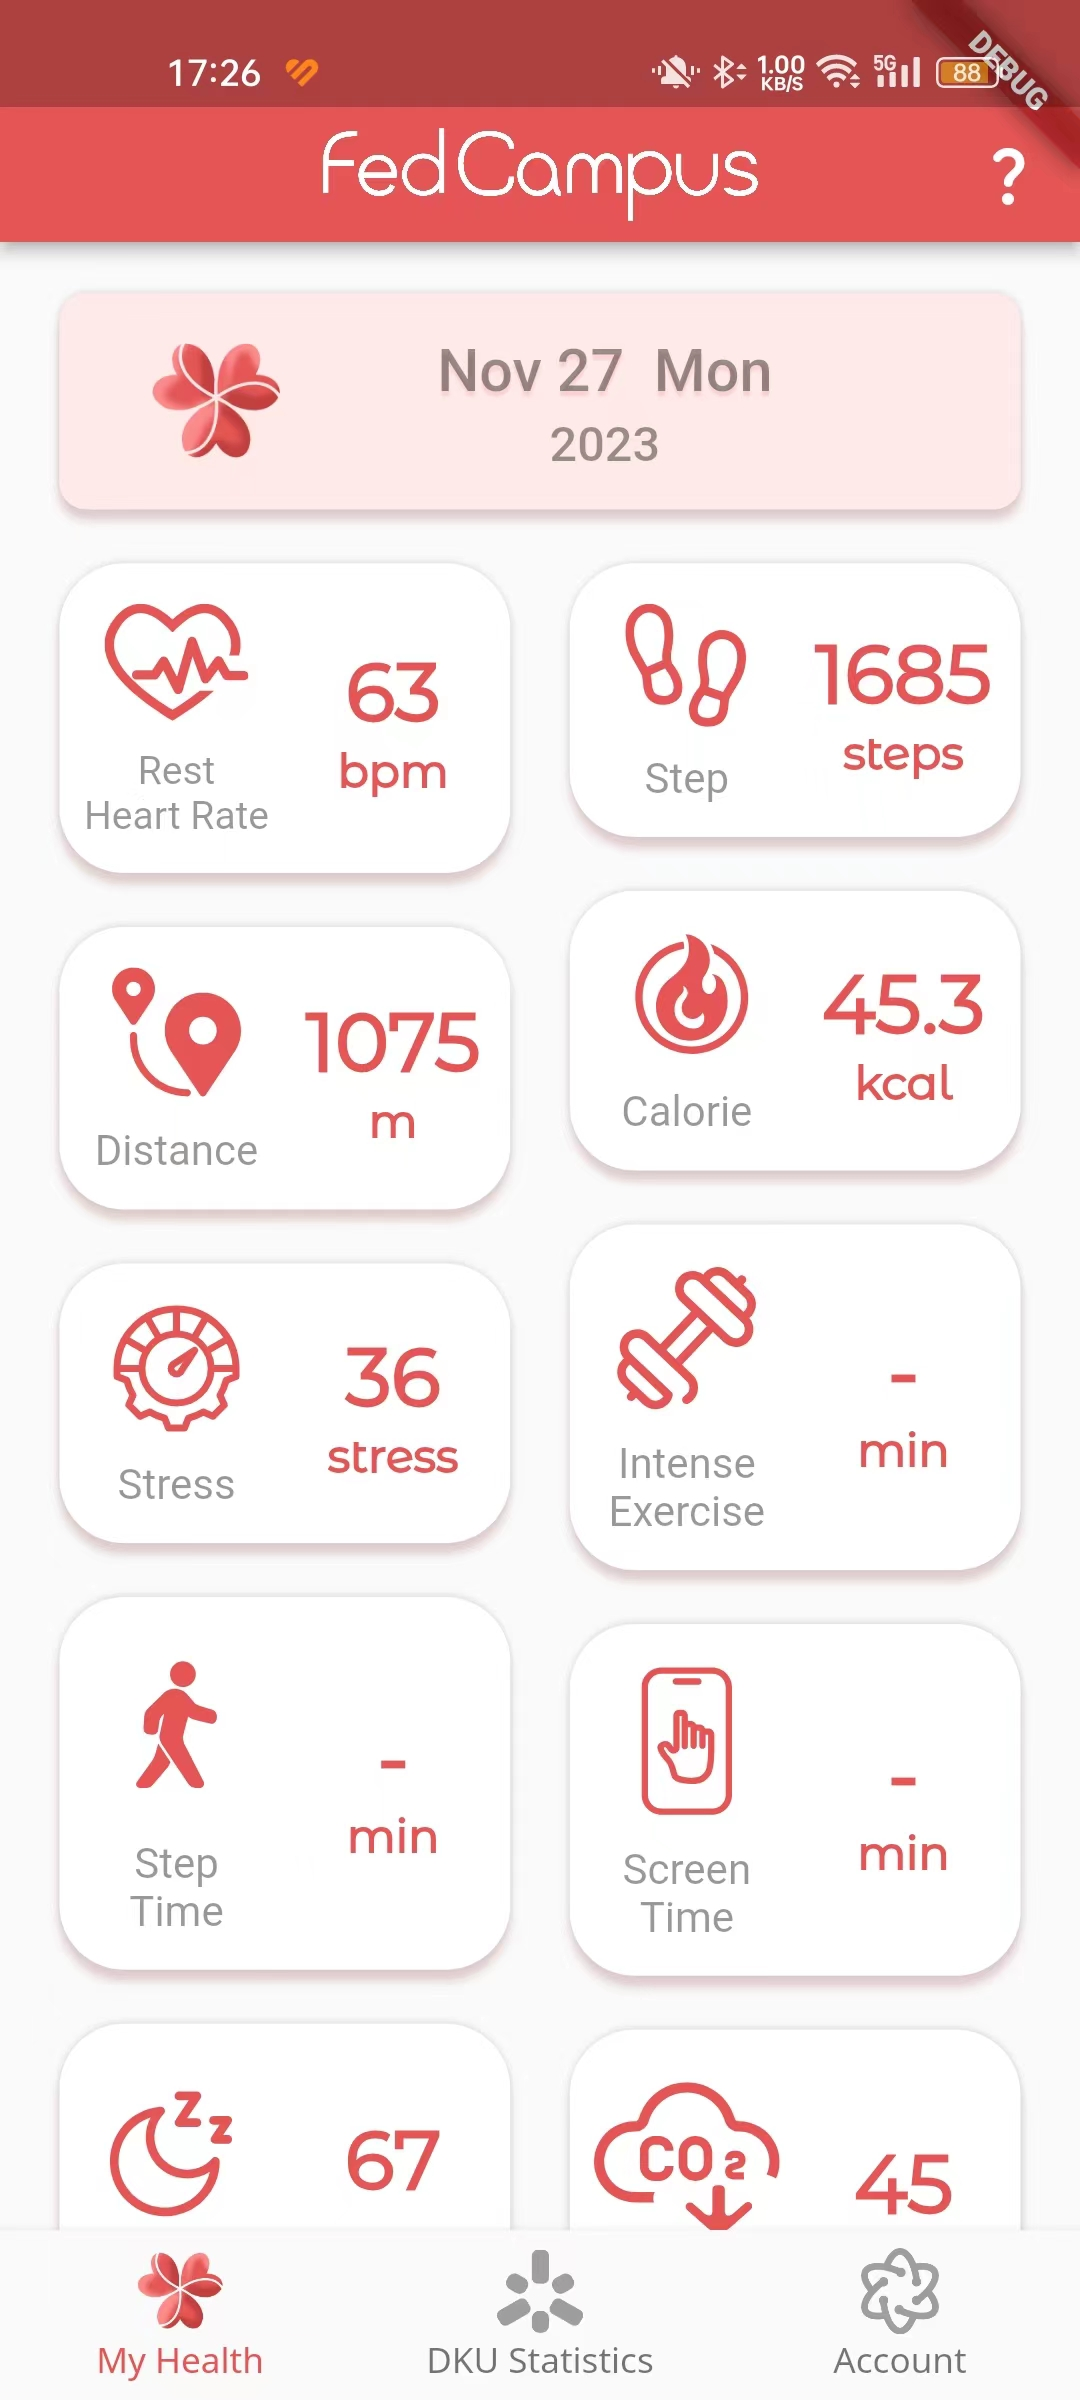
\includegraphics[width=0.3\linewidth]{fedcampus_screenshot1.jpeg}
        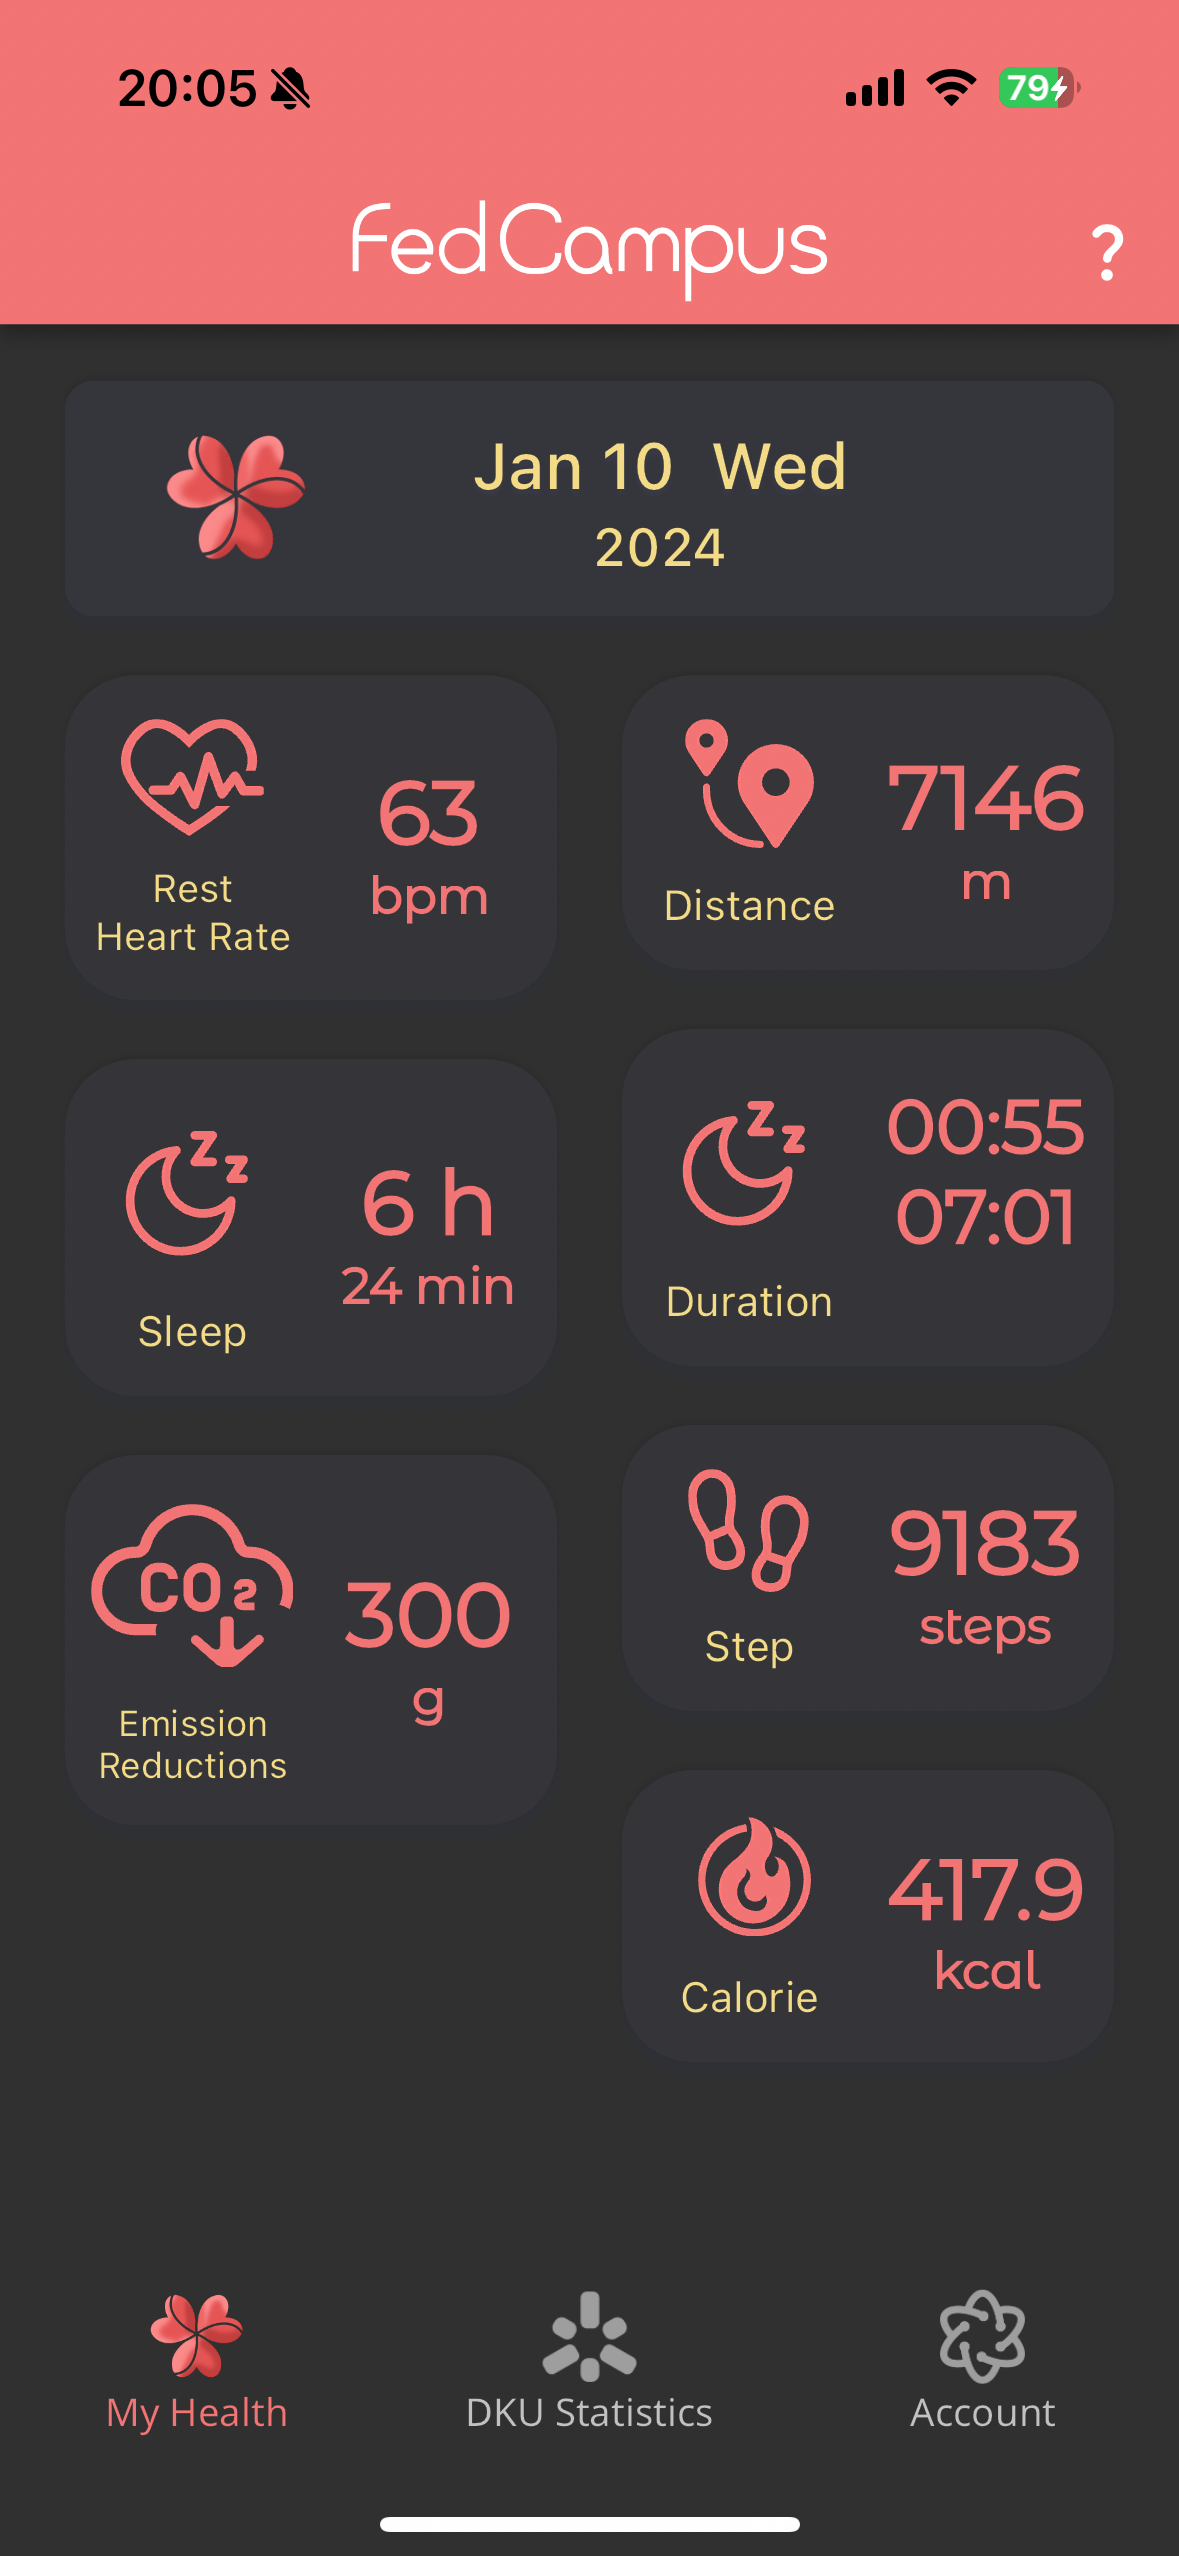
\includegraphics[width=0.31\linewidth]{fedcampus_screenshot3.png}
        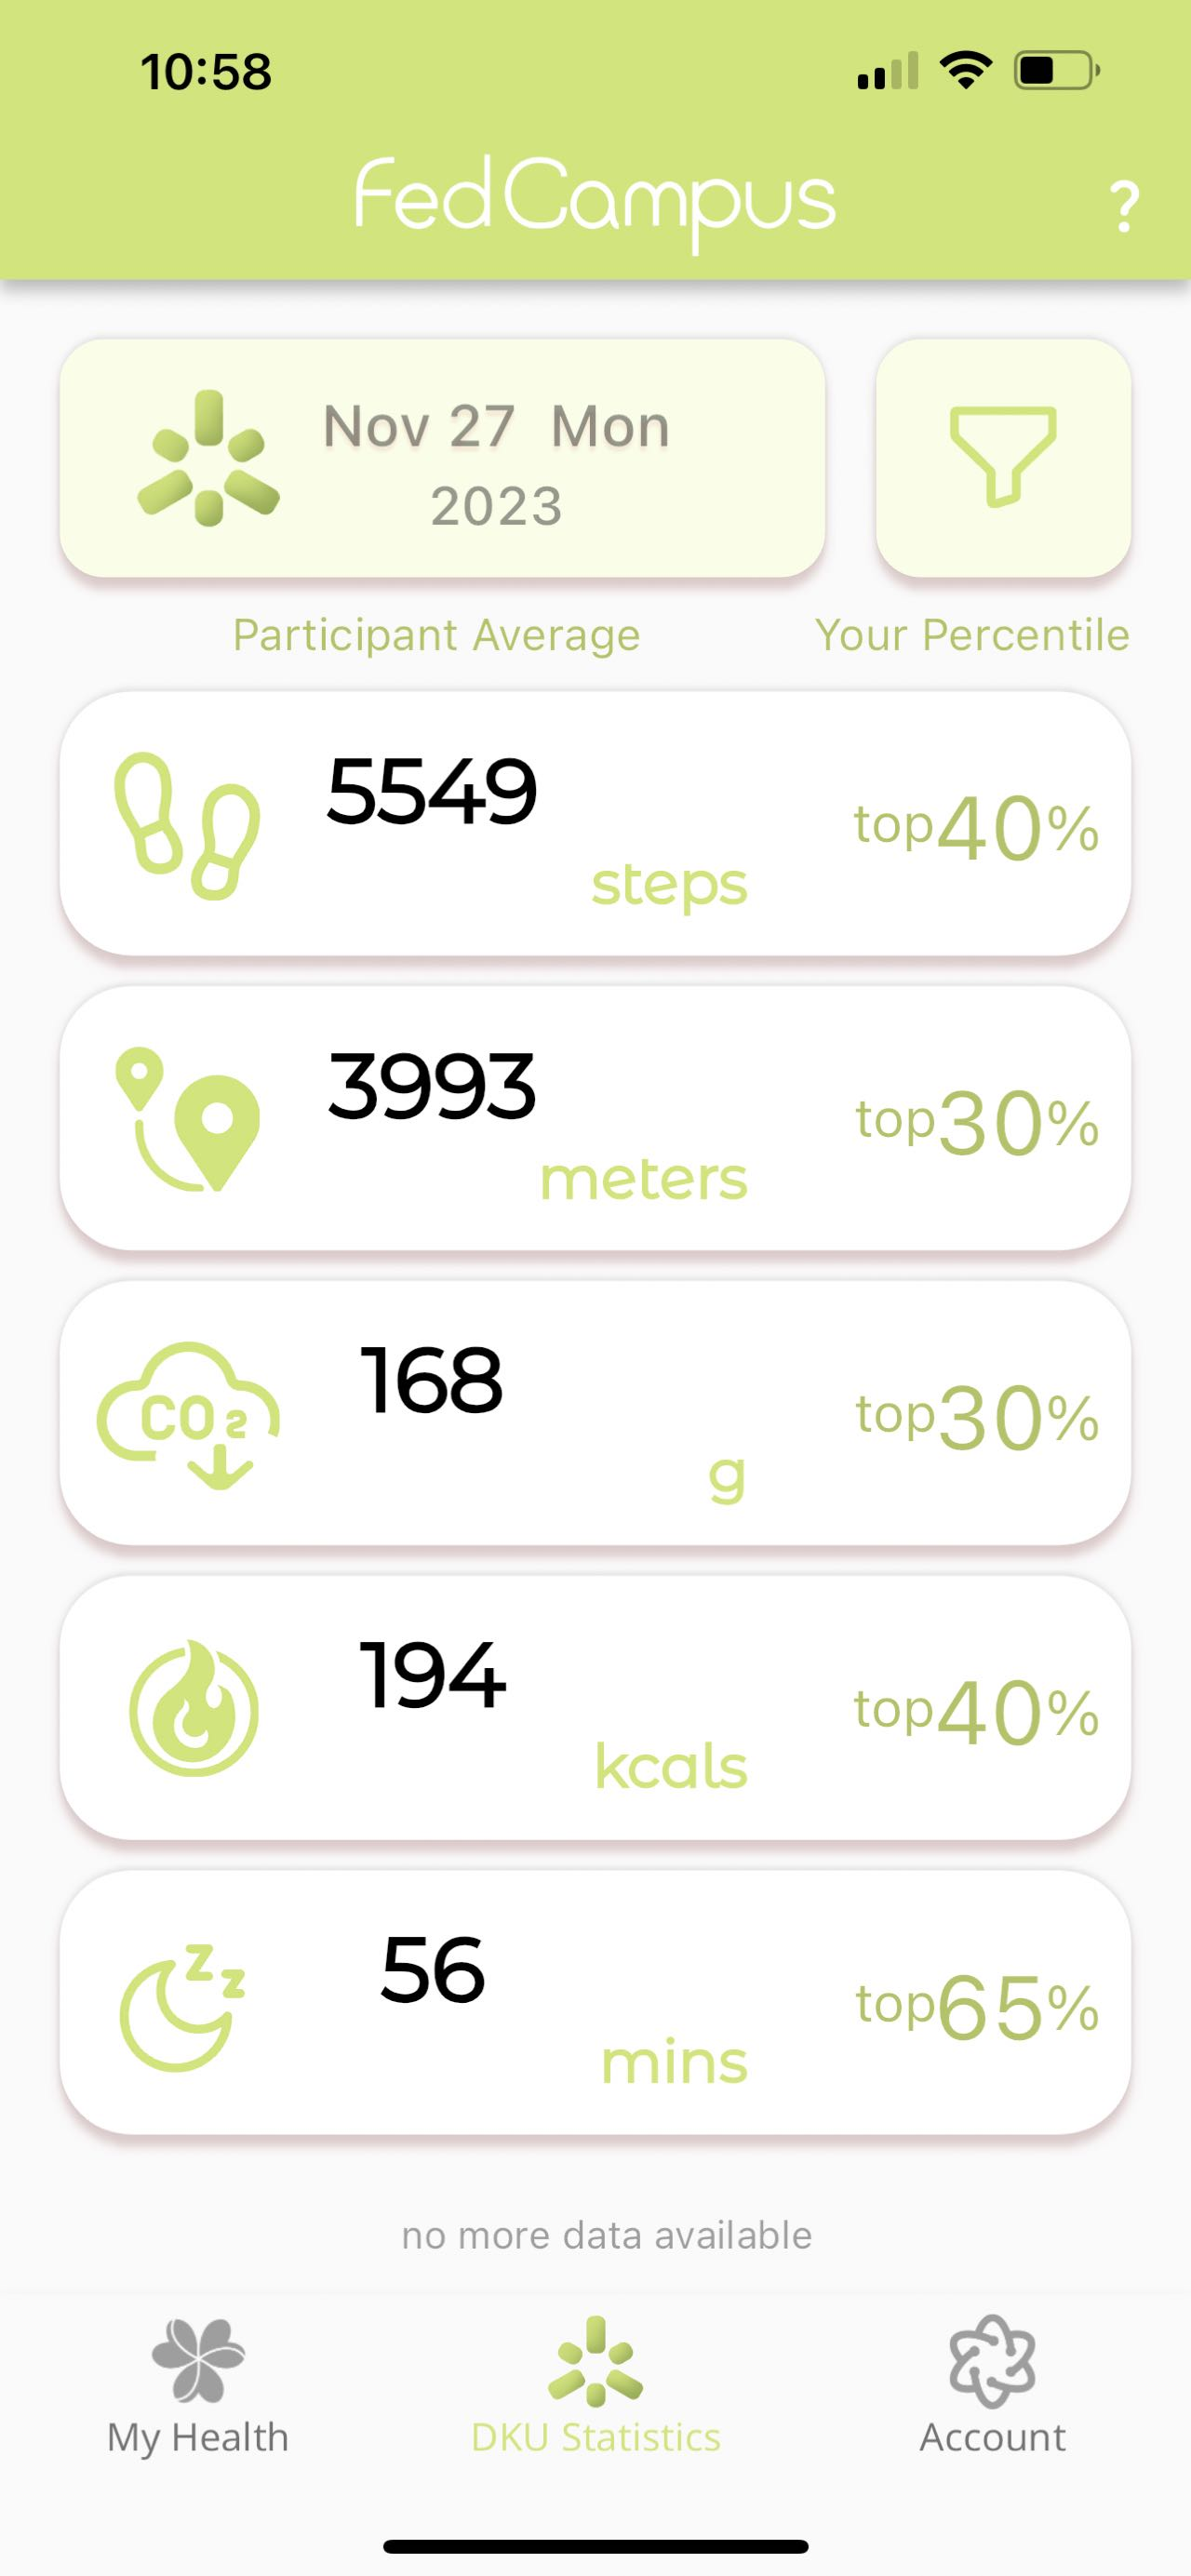
\includegraphics[width=0.31\linewidth]{fedcampus_screenshot2.jpeg}
        \caption{Screenshots of The \fedcampus Application.
            On The left, The User's Personal Health Page on Android;
            On The Middle, The User's Personal Health Page on iOS in Dark Mode;
            On The Right,
            The Group Mean And The User's Approximate Percentile Within The
            Group From Federated Analytics.
        }
    \end{center}\end{figure}

We launched the \fedcampus Application among Duke Kunshan University students,
faculty, and staff in November 2023.
At launch,
the \fedcampus Application displays the users' personal health data accessed,
as well as some statistics derived from federated analytics (see \ref{app:fa}),
as shown in Figure~\ref{fig:fedcampus-app}.
We offered the opportunity to participate in \fedcampus either by lending them
Huawei smartwatches or by using their own Huawei smartwatches.
The \fedcampus Application currently has 93 registered users and approximately
half of them are daily active users.

\subsection{\fedcampus Participant Requirements}

Our involved data access setup results in involved participant requirements.

In practice, accessing the data via the Huawei Health Kit on Android only works
well for participants using Huawei smartphones.
On Huawei smartphones,
the operating system automatically periodically synchronizes health data from
the connected Huawei smartwatch to the Huawei Health Kit.
Therefore, when these participants launch our FedCampus Application,
the app can immediately access the latest data from the Huawei Health Kit.

However, on non-Huawei Android smartphones,
the synchronization from the smartwatches only happens when
the Huawei Health app is on the foreground,
unless participants install Huawei Management System Core (HMS Core),
a background service app.
Alpha testers reported that the HMS Core is battery-consuming,
and is sometimes shut down by the operating system on smartphones made by
Xiaomi and other companies.
Additionally, Huawei apps are not available on the Google Play Store,
so some participants also have to install the Huawei AppGallery Application.
This makes an undesirable experience where the participants are required to
install four different apps.
Despite the inconveniences, once the participants have installed the apps,
they do not need to conduct this process again.

On iOS, participants can download the Huawei Health app from the App Store,
but it does not synchronize data from the Huawei smartwatch in the background.
Participants have to manually open the Huawei Health app,
and leave it in the foreground to synchronize the data both from
the smartwatches to the Huawei Health Kit,
and from the Huawei Health Kit to the Apple HealthKit.
It takes a significant amount of time for Huawei Health Kit to
synchronize the data to Apple HealthKit,
especially for the sleep time data;
as a result, it is common for the FedCampus Application to miss sleep data as
it could not read it from Apple HealthKit.

Due to these practical limitations,
we first prioritized Huawei smartphone users, then iPhone users,
for our initial launch.

\section{\fedkit Demonstrations}

To demonstrate \fedkit's capabilities,
we conducted two demonstrations~\cite{he2024fedkit}.
The first demonstration showcases \fedkit's federated learning model pipeline in
a lab setting,
and the second demonstration showcases \fedkit's integration in the \fedcampus
Application.

\subsection{\fedkit MNIST Demonstration}

\begin{figure}\begin{center}
        \label{fig:lab}
        \includegraphics[width=\linewidth]{mnist_demo_photo.jpeg}
        \caption{A previous \fedkit Demonstration Using A MNIST Model And
            Running on An Android Phone And An iOS Simulator.
        }
    \end{center}\end{figure}

We demonstrate federated learning among
devices running an example Flutter client app,
and a laptop running a \fedkit Backend. Each client has $\frac{1}{10}$ of the
MNIST~\cite{cohen2017emnist} dataset locally,
which is used to participate in the federated learning process.

First, we demonstrate our seamless federated learning model pipeline.
We convert a TensorFlow MNIST multi-layer perceptron model and
conduct federated learning with it across an Android and an iOS device.
A previous demonstration running this model is shown in Figure~\ref{fig:lab}.
Second, to showcase machine learning model operations,
we modify the model and deploy its new version.
As outlined in Table~\ref{tbl:demo-stats},
our telemetry shows that
the iOS device is over 5$\times$ faster in local training despite
having 0.5$\times$ RAM,
illustrating how \fedkit will provide real-world statistics to
enhance federated learning algorithm design.

\begin{table}\begin{center}
        \begin{tabular}{lllll}\toprule
            Device            & System on a Chip  & Acceleration & RAM         & Time   \\\midrule
            Huawei Nova 9 Pro & Snapdragon 778G   & OpenCL       & 8GB LPDDR5  & 3.583s \\
            iPhone 13 mini    & A15 Bionic, 4 GPU & CoreML       & 4GB LPDDR4X & 0.656s \\\bottomrule
        \end{tabular}
        \caption{Configurations of Devices and Average Local Training Time Per Round
            (Two Local Epochs) in A Previous Demo Run.
        }
        \label{tbl:demo-stats}
    \end{center}\end{table}

\subsection{\fedkit Integration in The \fedcampus Application}

\begin{figure}\begin{center}
        \label{fig:integration}
        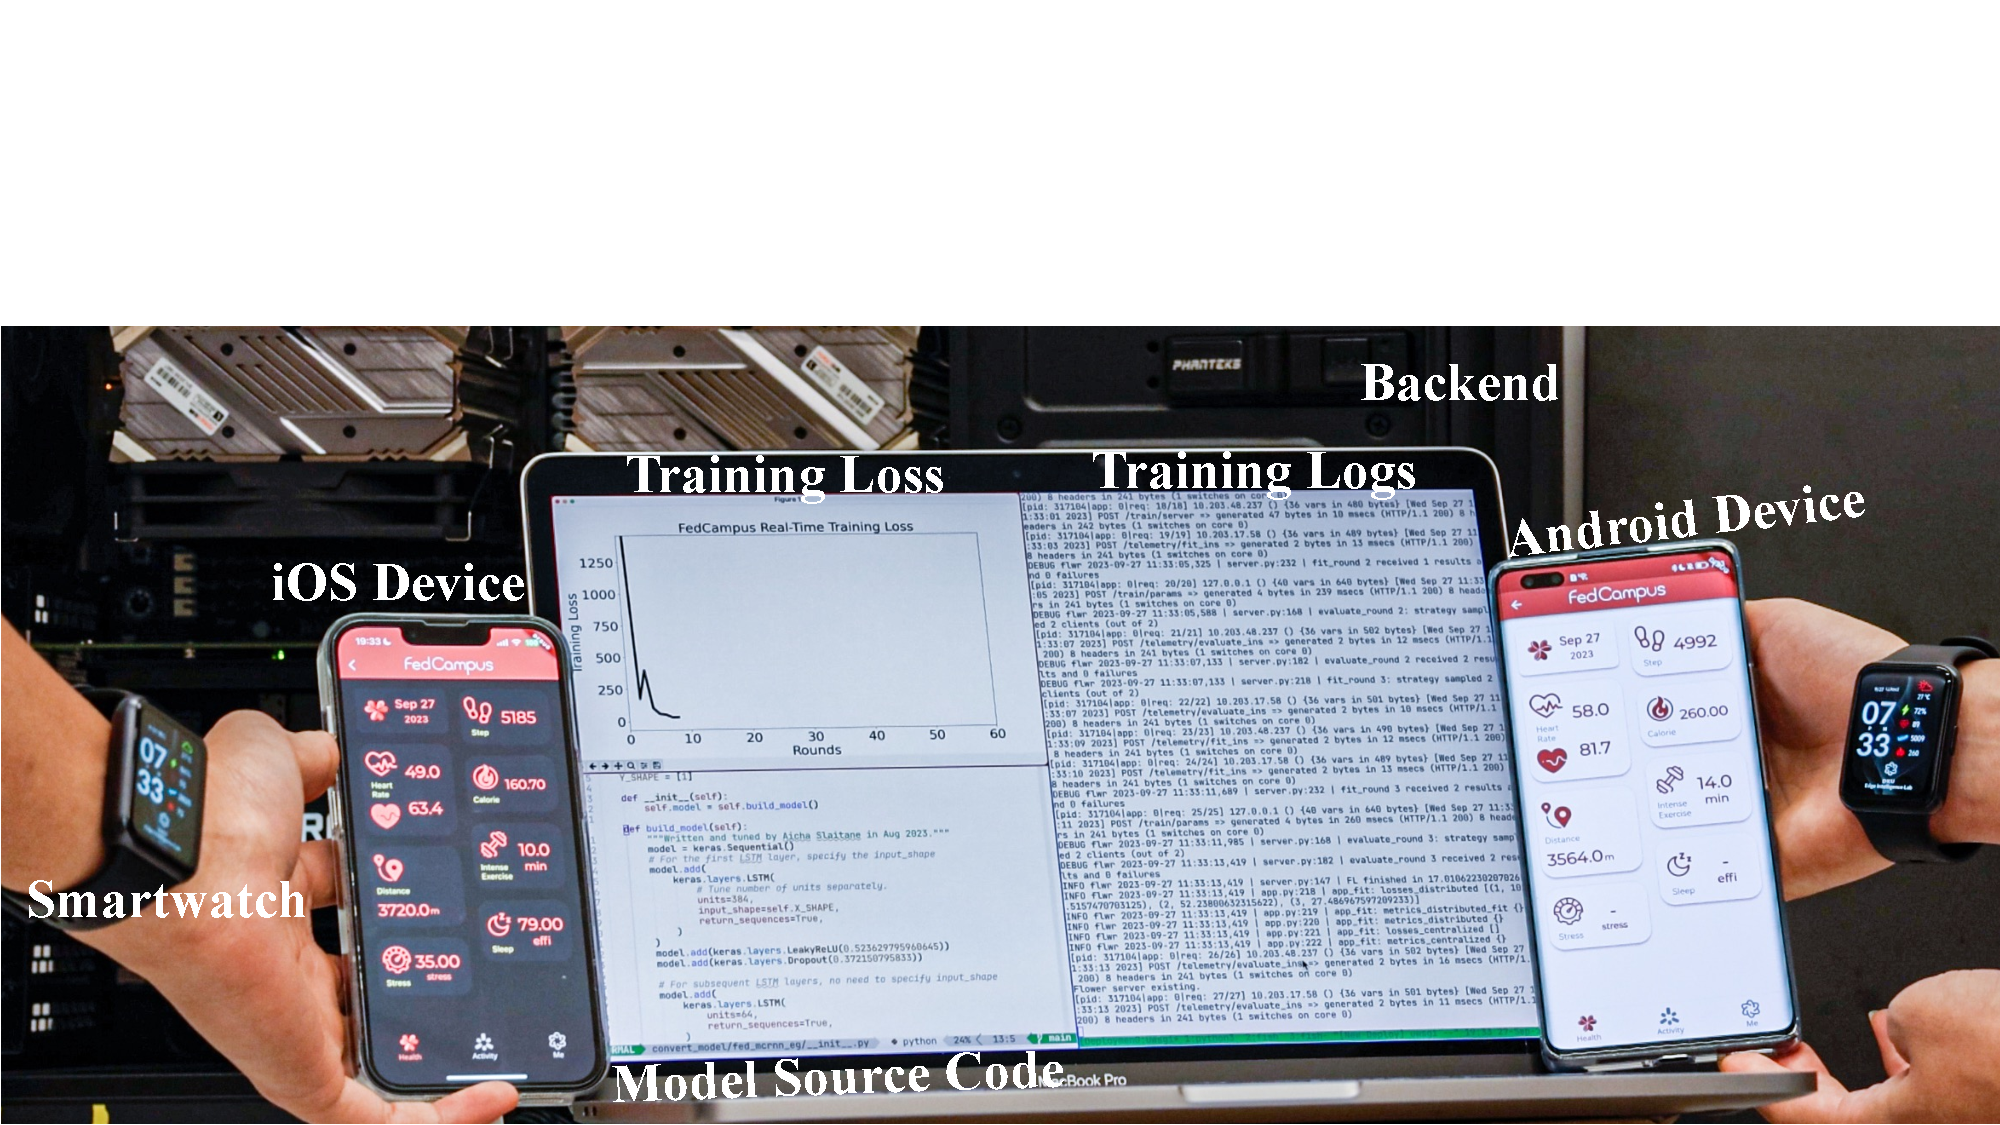
\includegraphics[width=\linewidth]{fedcampus.pdf}
        \caption{Experiment Setup for The \fedkit Integration in The FedCampus
            Application.
        }
    \end{center}\end{figure}

We integrated \fedkit into the \fedcampus Application to
conduct a federated learning experiment using health data on the smartphones,
as displayed in Figure~\ref{fig:integration}.
In our setup,
A backend server is hosted in the physical machine in the background,
while an Android device and an iOS device are running an early version of
the \fedcampus Application.
The laptop is connected to the server via Secure Shell (SSH),
and was displaying the training logs,
along with the training loss and the model's source code.

The \fedcampus Application in this experiment trained a sleep-efficiency
prediction model similar to the model described in~\cite{khoa2022fedmcrnn}
using health data collected from the smartwatches.
Each round of training is instantaneous on both Android because of
the small training dataset,
and both smartphones remained cool with \fedkit's training acceleration.
The models trained on these smartphones are aggregated across Android and iOS,
resulting in a significant reduction in the training loss,
demonstrating \fedkit's effectiveness in real-world scenarios.
